
\chapter{Tesstování a evaluace}

V této kapitole je popsáno jak je celá aplikace otestována. Dále pak porovnání odhadů zpoždění se stávajícím řešení.

\section{Testování softwarového řešení}

Ko'd práce popsaný v kapitole \ref{chapter:implementace} je otestován unit testy. Propojení  tohoto softwaru s databází i zdrojem vstpuních dat je testováno integračními testy.

\subsection{Unit testy}

Unit testy testují spravnou funkčnost jednotlivých metod všech softwarových komponent této práce.

Pro ověření správné funkčnosti některých metod jsou vygenerována vstupní či výstupní data. To z důvodu, že tyto metody pracují z komplexní datovou strukturou nebo s velkým objemem dat, který není možno zadat jako vstupní přímo v ko'du testu, resp. je potřeba porovnat výstup tetované metody a ze stejných důvodů není možné uvádět výstupní hodnoty pro porovnání přímo v ko'du testu. Typickým příkladem takové vstupní struktury je model profilu jízdy, ptotože je potřeba otestovat funkce, které s takovým modelem pracují.

\subsection{Integrační testy}

TODO Popisovat co testují testy? Není v tom žádná složitá logika. Dále otázka k celému textu jak odkazovat na jednotlivé soubory s kodem?

\subsection{Výkonostní testy}

Všechny následující výkonostní testy jsou prováděny na osobním notebooku s technickými parametry uvedenými v tabulce \ref{table:hw}', kde všechny procesy aplikace včetně databáze běží paralelně.

\begin{center}
	\begin{table}[ht]
\centering
\begin{tabular}{|c|c|}
\hline
 Parametr & Hodnota \\ \hline \hline
 Procesor & 4x Intel(R) Core(TM) i7 CPU @ 2.70 GHz\\ \hline
 Pamětˇ & 16 GB DDR3 RAM  \\  \hline
 Rychlost zápisu na disk & 1000--3000 MB/Sec \\ \hline
 OS & macOS Big Sur\\ \hline
 MySQL & version 8.0.18\\ \hline
\end{tabular}
\label{table:hw}
\end{table}
\end{center}
\footnote{https://9to5mac.com/2016/11/01/the-late-2016-entry-level-13-macbook-pro-has-a-ridiculously-fast-ssd/}
\bigbreak

Pro potlačení zkreslení testů vlivem čekání na stažení dat z internetu jsou všechny data načítána z disku počítače.

\bigbreak

Testování stejně jako funkční a kvalitativní požadavky na práci vychází z analýzy vstupních dat uvedené v kapitole \ref{subsubsection:vstupni_soubory}.

\subsubsection{Zpracování dat}

Zpracování dat probíhá přečtením souboru s polohy vozidel a dále zpracovává každé vozidlo zvláštˇ. Přičemž pokud je vozdilo již nalezeno a jeho poloha se od poslední aktualizace změnila provedou se pouze 2 čtení z databáze, jeden záznam se aktualizuje a vloží se jeden nový záznam. Pokud je vozdilo již nalezeno a jeho poloha se od poslední aktualizace nezměnila provedese se pouze jedno čtení z databáze. Pokud ovšem je vozidlo obsluhující spoj nenalezeno musí se číst soubor s detailem daného spoje a všechna data se vkládají do databáze (jízdní řád včetně zastávek) navíc geografická lomená čára popisující jízdu se ukládá jako soubor.

\bigbreak

Jak je ale vidět na grafu \ref{fig:file_process_time} i pro nejvyšší množství vozidel (720) celé zpracování trvá nanejvýš 1.2 sekundy. Z toho plyne, že samotné zpracování dat není nijak časově náročné a vzhledem k 20sekundové periodě aktulizace dat máme velkou časovou rezervu. Rychlost zpracování jednoho vstupního souboru může více ovlivnit stahování dat z internetu, kde ale předpokládáme, že po většinu času nebude trvat stáhnout aktuální polohy vozidel déle než desítky milisekund.

\bigbreak

\begin{figure}
	\centering
  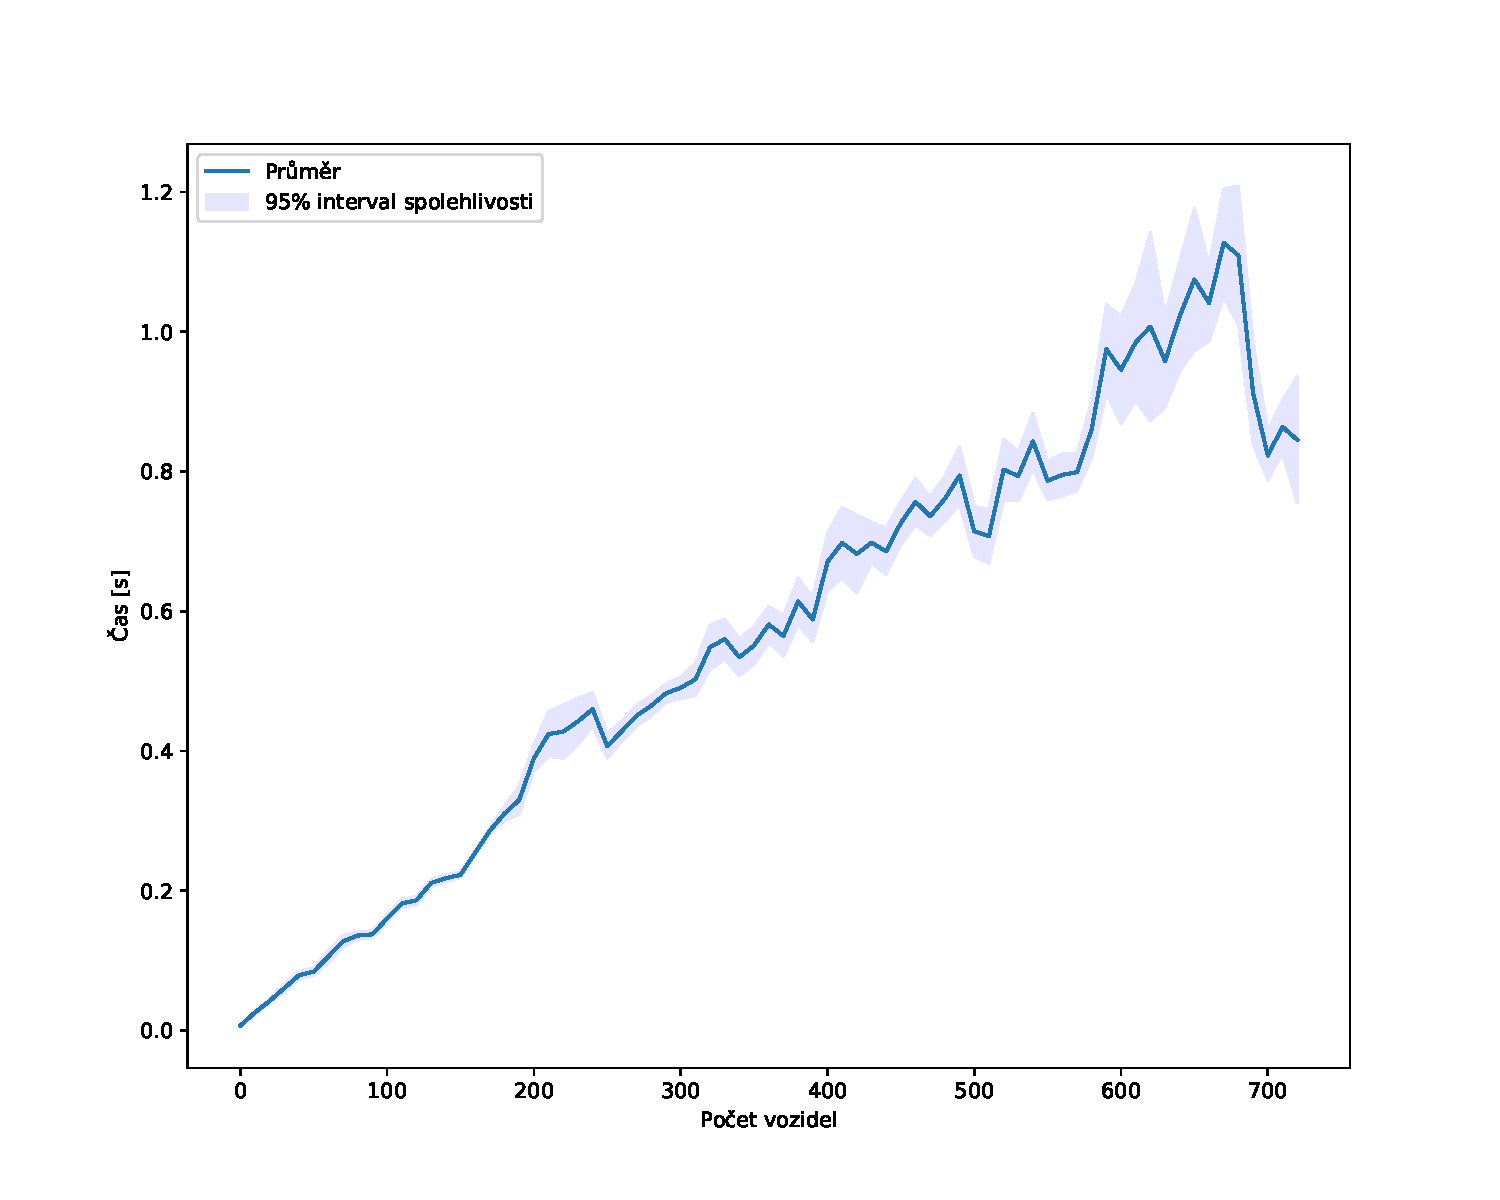
\includegraphics[width=0.7\linewidth]{../img/file_process_time}
  \caption{Průměrný čas zpracovávání daného počtu vozidel ze všech souborů se statickými daty. Světle modrá barva ohraničuje 95 \% interval spolehlivosti. Počty vozidel jsou vždy zaokrouhleny dolů na celé desítky.}
  \label{fig:file_process_time}
\end{figure}

\bigbreak

Jediné delší prodlení může nastat ve chvíli, kdy je potřeba stáhnout velké množství dodatečných informací o novém spoji. Na grafu \ref{fig:vehicle_pos_x_new_trips} je vidět, že až na jednotky vyjímek je počet nově nalezených spojů v jednom souboru nejvýše 20. Aplikace je ale naimplementována tak, aby se tyto informace stahovaly asynchroně a tedy čákání na stažení dat je co nejkratší.

\subsubsection{Konstrukce modelů}

Čtení dat potřebných pro trénování modelů z databáze, kde jsou data ze 4 dnů trvá přibližně 110 sekund. Čtení se totiž provádí komlikovaným \gls{sql} datazem uvedeným v kapitole \ref{subsection:cteni_dat}, ovšem na rychlost provedení tohoto dotazu i konstrukce modelů celkem neklademe žádné časové nároky, protože přepočítávání modelů je plánováno na čas nejmenšího zatížení systému, což bývá typicky v noci, kdy máme několik hodin pro výpočet.

\bigbreak

Dále ověřme, že výsledek dotazu nezahltí pamětˇ počítače, dotaz sice umožnˇuje čtení dat po stránkách, ale v implementaci se tato vlastnost nevyužívá. Určení velikosti objektu jazyka Python3 v paměti počítače není úplně trivální úloha, dobrý odhad nám, ale poskytne objektu na disk pomocí knihovny \verb-pickle-. Takto uložený objekt zabírá necelých 10 MB prostoru na disku.

\bigbreak



\section{Evaluace výsledků}

\subsection{Sestrojení modelů}

Po využití testovacích dat vzorků poloh vozidel zaznamenaných ve dnech 20.--24. února 2020 bylo podle krytérií, kterými jsou zejména vzdálenost zastávek a počet vzorků mezi nimi, sestrojeno celkem 1106 polynomiálních modelů. Z toho je 847 modelů pro pracovní dny, které jsou nejdůležitější. Přičemž celkový počet párů zastávek je 7230, ale zastávek ve vzdálenosti 1500 metrů\footnote{zvolená minimální vzdálenost mezi zastávkama, mezi kterýma má ještě smysl odhadovat zpoždění} je pouze 2142. Z toho vychází, že u 40 \% dvojic zastávek je dostatek dat, aby dával výpočet modelu smysl.

\bigbreak

U zbylých dvojic zastávek se využívá lineární model.

\subsection{Odhady zpoždění}

Z toho jak jsou definovány požadavky řešení v kapitole \ref{subsubsection:kvalitativni_pozadavky} pro změření kvality výsledků stačí porovnávat odhad zpoždění lineárního (původního) modelu a nového polynomiálního modelu. Přičemž odhad je lepší pokud má sekvence odhadů  z celé jízdy mezi dvojcí zastávek menší rozptyl.

\bigbreak

Podívejme se tedy na porovnání odhadů zpoždění novými modely profilů jízd se stávajícím řešení pracujícím s předpokladem, že vozidla jedou celou trasu mezi dvěma zastávkami konstantní rychlostí.

\bigbreak

Evaluaci výsledků budeme provádět s daty sesbíranými 20. 2. 2020, které použijeme jako trénovací data a s daty sesbíranými 21. 2. 2020, které použijeme jako testovací data. Toto je standardní postup pro hodnocení úspěšnosti predikcí modelů ve světě strojového učení. Modely nemohou být testovány na stejných datech jako na kterých byly trénovány, protože kdyby se trénovalo i testovalo na stejných datech, model by nemusel nic predikovat, ale stačilo by, aby si jen "zapamatoval" hodnotu z množiny trénovacích dat.

\bigbreak
